%************************************************
\chapter{Invertible Networks}\label{invertible-networks}
%**************************************

\begin{startbox}{Invertible networks can help understand learned discriminative features in the EEG}
\item Class prototypes can be visualized
\item Per-electrode prototypes may be even more interpretable
\item Additionally, a small interpretable network may allow further insights
\end{startbox}


Invertible networks are networks that are invertible by design, i.e.,
any network output can be mapped back to a corresponding input
bijectively \citep{DBLP:journals/corr/DinhKB14,DBLP:journals/corr/DinhSB16,DBLP:conf/nips/KingmaD18,DBLP:conf/icml/RezendeM15,DBLP:conf/icml/HoCSDA19}.
The ability to invert any output back to the input enables different
interpretability methods and furthermore allows training invertible
networks as generative models via maximum likelihood.

This chapter starts by explaining invertible layers that are used to
design invertible networks, proceeds to detail training methodologies
for invertible networks as generative models or classifiers, and goes on
to outline interpretability techniques that help reveal the learned
features crucial for their classification tasks.

\section{Invertible Layers}\label{invertible-layers}

    Invertible networks use layers constructed specifically to maintain
invertibility, thereby rendering the entire network structure
invertible. Often-used invertible layers are coupling layers, invertible
linear layers and activation normalization layers
\citep{DBLP:conf/nips/KingmaD18}.

\textbf{Coupling layers} split a multidimensional input $x$ into two
parts $x_1$ and $x_2$ with disjoint dimensions and then use $x_2$
to compute an invertible transformation for $x_1$. Concretely, for an
additive coupling layer, the forward computation is:


\begin{align*}
    y_1 &= x_1 + f(x_2) && \codecomment{\text{Compute } y_1 \text{ from } x_1 \text{ and arbitrary function f of } x_2} \\
    y_2 &= x_2 && \codecomment{\text{Leave } x_2 \text{ unchanged}} \\
\intertext{The inverse computation is:}
    x_1 &= y_1 - f(y_2) && \codecomment{\text{Invert to } x_1 \text{ using unchanged } y_2=x_2} \\
    x_2 &= y_2 &&  \codecomment{x_2 \text{ was unchanged}}\\
\end{align*}

% 

For the splitting of the dimensions in a timeseries, there are multiple
ways, such as using the even time indices as $x_1$ and all the odd
time indices as $x_2$ or using difference and mean between two
neighbouring samples (akin to one stage of a Haar Wavelet). The function
$f$ is usually implemented by a neural network, in our cases it will
be small convolutional networks. Instead of addition any other
invertible function can be used, affine transformation are commonly
used, where $f$ produces translation and scaling coefficients $f_t$
and $f_s$:
\begin{align*}
    y_1 &= x_1 \cdot f_s(x_2) + f_t(x_2) && \text{ } y_2=x_2 && \codecomment{\text{Affine Forward }} \\
    \\
    x_1 &= \frac{(y_1  - f_t(y_2))}{f_s(y_2)} && \text{ } x_2=y_2 && \codecomment{\text{Affine Inverse}} \\
\end{align*}

\textbf{Invertible linear layers} compute an invertible linear
transformation (an automorphism) of their input. Concretely they
multiply a $d$-dimensional vector $\mathbf{x}$ with a
$dxd$-dimensional matrix $W$, where $W$ has to be invertible,
i.e., have nonzero determinant.

\begin{align*}
    y&=W \mathbf{x} && \codecomment{\text{Linear Forward }} \\
    x&=W^{-1} \mathbf{y} && \codecomment{\text{Linear Inverse}} \\
\end{align*}

For multidimensional arrays like feature maps in a convolutional
network, these linear transformations are usually done per-position, as
so-called invertible 1x1 convolutions in the 2d case.


\textbf{Activation normalization layers} perform an affine
transformation with learned parameters with $s$ and $t$ learned
scaling and translation parameters (independent of the input $x$):

\begin{align*}
    y&=x \cdot{s} + t && \codecomment{\text{ActNorm Forward}} \\
    x&=\frac{y - t}{s} && \codecomment{\text{ActNorm Inverse}} \\
\end{align*}

These have also been used to replace batch normalization and are often
initialized data-dependently to have standard-normalized activations at
the beginning of training.


\section{Generative Models by Maximizing Average Log
Likelihood}\label{generative-models-by-maximizing-average-log-likelihood}

    Invertible networks can also be trained as generative models via
maximizing the average log likelihood. In this training, the network is
optimized to maximize the average log probabilities of the training
inputs, which is equivalent to minimizing the Kullback-Leibler (KL)
divergence between the training distribution and the learned model
distribution \cite{DBLP:journals/corr/TheisOB15}. Invertible
networks assign probabilities to training inputs $x$ by mapping them
to a latent space $z=f(x)$ and computing their probabilities under a
predefined prior $p_z(z)$ in that latent space. For real-valued
inputs, one has to account for quantization and volume change to ensure
this results in a proper probability distribution $p_x$ in the input
space. Quantization refers to the fact that training data often consists
of quantized measurements of underlying continuous data, e.g.~digital
images can only represent a distinct set of color values. Volume change
refers to how the invertible networks' mapping function $f$ expands or
squeezes volume from input space to latent space.

\subsection{(De)quantization}\label{dequantization}
    
\begin{figure}[ht]
    \myfloatalign
    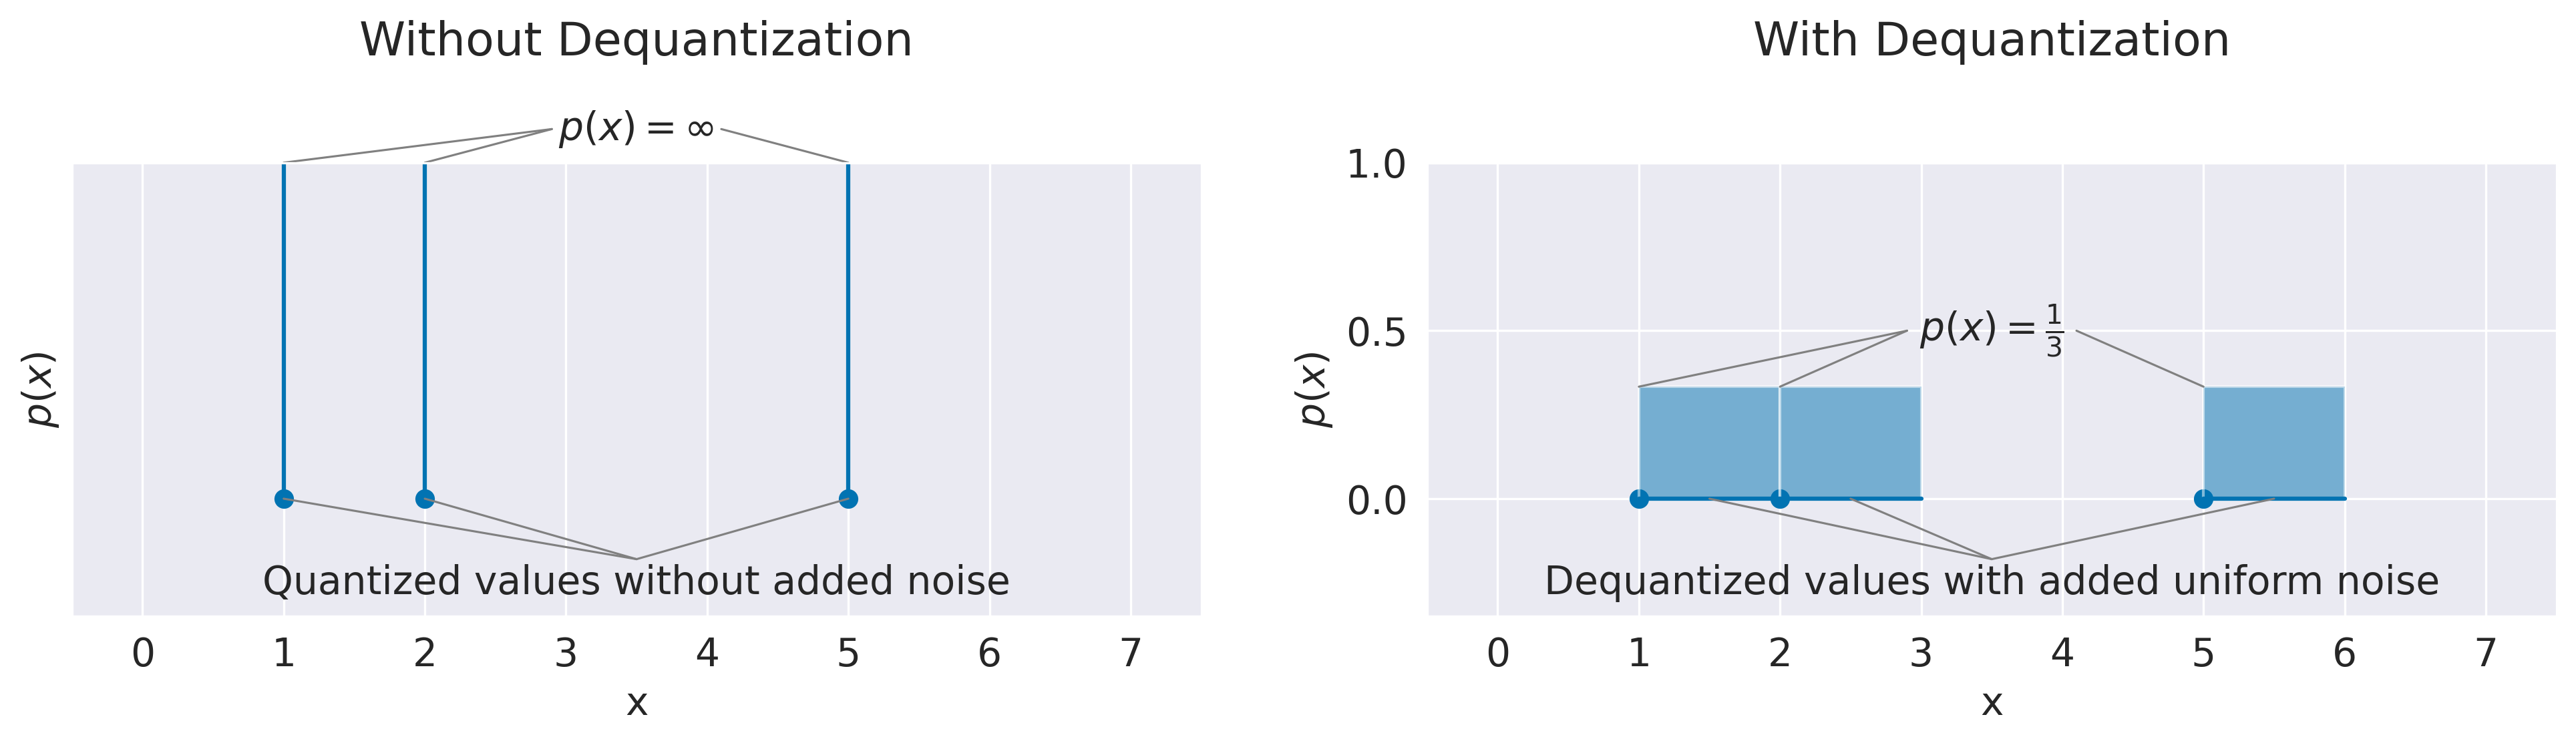
\includegraphics[width=1\linewidth]{images/dequantization.png}
    \caption[Average log-likelihood-maximizing distributions without and with
dequantization]{
\textbf{Average log-likelihood-maximizing distributions without and with
dequantization.} Examples show result of fitting quantized values like
discrete integer color values with a continuous probability
distribution. Example training distributions have 3 data points at
$x_1=1$, $x_2=2$ and $x_3=5$. On the left, fitting quantized
values directly leads to a pathological solution as the learned
distribution $p$ can assign arbitrarily high probability densities on
the data points. On the right, adding uniform noise $U(0,1)$ to the
datapoints leads to a distribution that also recovers the correct
discrete distribution, that means integrating over the probability
densities in the volume of each point leads to $P(x_i)=\frac{1}{3}$.
}
\label{dequantization-fig}
\end{figure}

    

    Often, training data for neural networks consists of quantized
measurements like discrete integer color values from 0 to 255, which are
mapped to real-world floating point numbers for training. Naively
maximizing the average log probability densities of these quantized
values with a continuous probability distribution would lead to
pathological behavior as the quantized training data points do not cover
any volume. Hence it would be possible for the learned distribution to
assign infinitely high probability densities to individual data points,
see \Cref{dequantization-fig} for an illustration.

Hence, one needs to ``dequantize'' the data such that each datapoint
occupies volume in the input space
\citep{DBLP:journals/corr/DinhSB16,DBLP:conf/icml/HoCSDA19}.
The simplest way here is to add uniform noise to each data point with a
volume corresponding to the gap between two data points. For example, if
the 256 color values are mapped to 256 floating values between 0 and 1,
one may add uniform noise $u\sim(0,\frac{1}{256})$ to the inputs. Then
the KL-divergence between the dequantized continuous distribution and
the learned continuous distribution is upper bounded by the
KL-divergence between the underlying discrete distribution and the
learned discrete distribution obtained by integrating over the noise
samples for each input \citep{DBLP:journals/corr/TheisOB15}.
Since in our case, we are not primarily interested in the exact
performance as a generative model in terms of number of bits, we simply
add gaussian noise with a fixed small standard deviation $N(0,0.005I)$
during training.

\subsection{Volume Change}\label{volume-change}

\begin{figure}[ht]
    \myfloatalign
    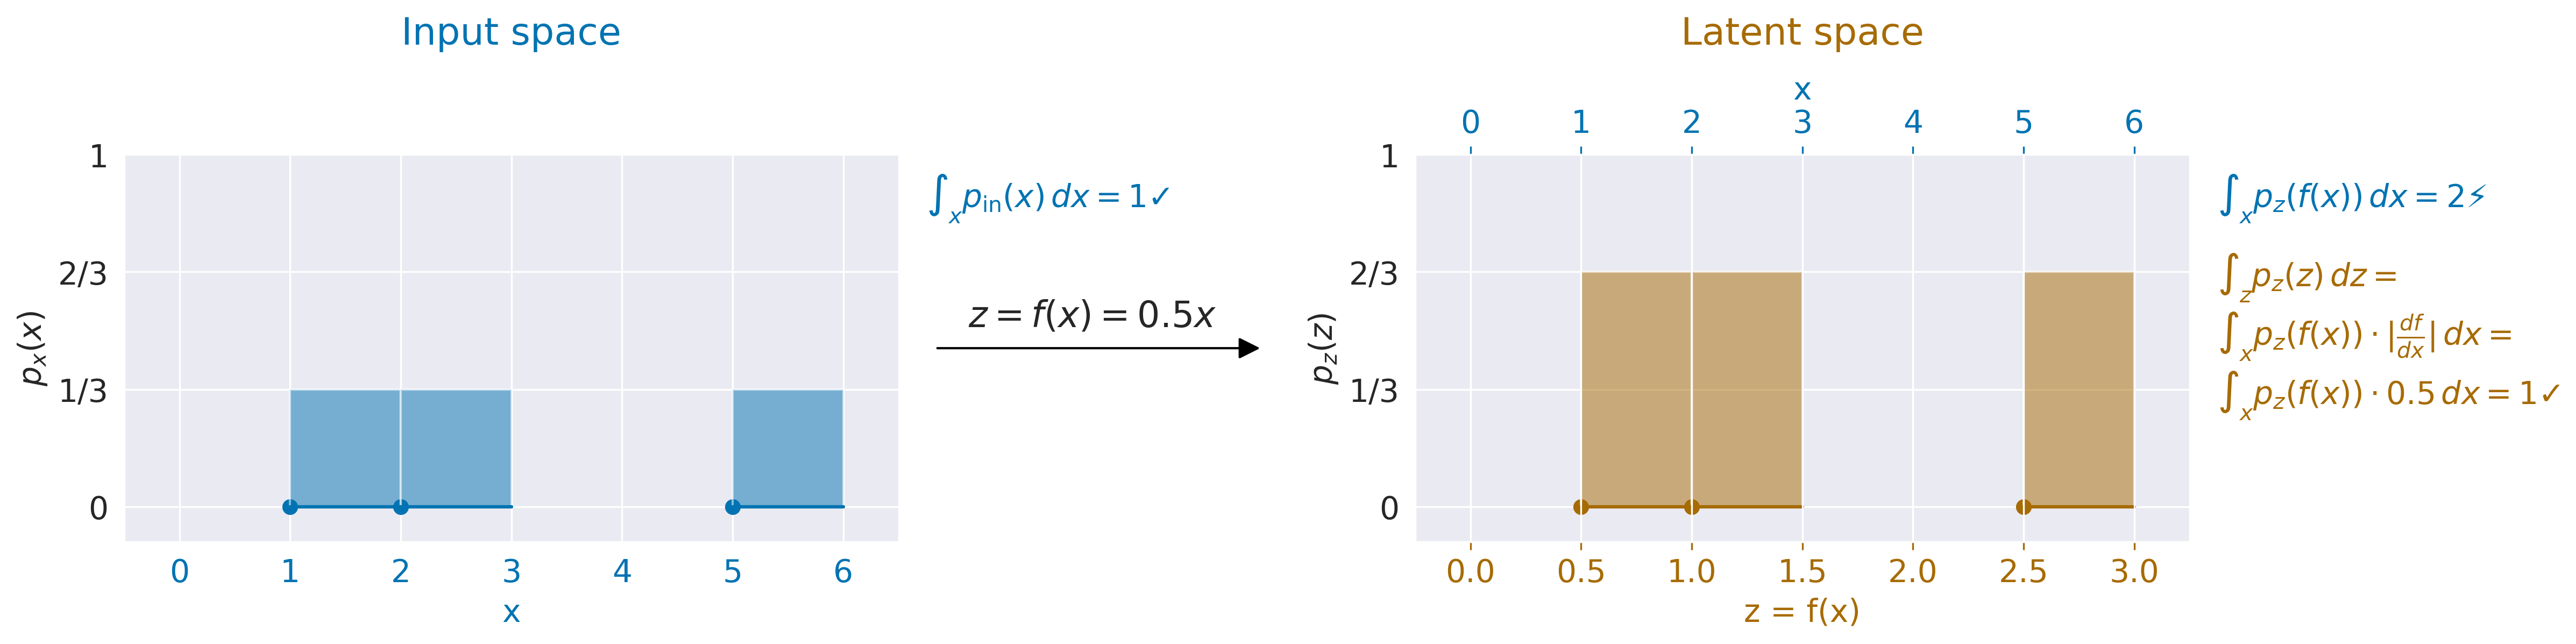
\includegraphics[width=1\linewidth]{images/change-of-volume.png}
    \caption[Volume change illustration]{
\textbf{Probability densities and volume changes.} Computing probability densities taking into account how a mapping function changes volume. Input $x$ with probability distribution $p_\text{x}(x)$
on the left is scaled by 0.5 to $z=f(x)=0.5x$ with probability
distribution $p_\text{z}(z)$ on the right. Naively integrating
$p_\text{z}(f(x))$ over x would lead to a non-valid probability
distribution with $\int_x p_\mathrm{z}(f(x)) \, dx=2$. To get the
prober probability densities in input space from $p_\text{z}(z)$, one
has to multiply with the volume changes, in this case the scaling factor
of the mapping $f(x)$ from x to z, giving
$p_\text{x}(x)=p_\mathrm{z}(f(x)) \cdot \frac{df}{dx}=p_\mathrm{z}(f(x))\cdot 0.5$
which correctly integrates to 1.
}
\label{change-of-volume-fig}
\end{figure}



    In addition, for these probability densities in latent space to form a
valid probability distribution in the input space, one has to account
for how much the network's mapping function squeezes and expands volume.
Otherwise, the network can increase densities by squeezing all the
inputs closely together in latent space, see also
\Cref{change-of-volume-fig} for a onedimensional example. To
correctly account for the volume change during the forward pass of $f$
one needs to multiply the probability density with the volume change of
$f$, descreasing the densities if the volume is squeezed from input to
latent space and increasing it if the volume is expanded. As the volume
change at a given point $x$ is given by the absolute determinant of
the jacobian of f at that point
$\det \left( \frac{\partial \mathbf{f}}{\partial \mathbf{x}} \right)$,
the overall formula looks like this:

\begin{align}
p(x) = p_\textrm{z}(f(x)) \cdot | \det \left( \frac{\partial \mathbf{f}}{\partial \mathbf{x}} \right)|
\end{align}

Or in log-densities:

\begin{align}
\log p(x) = \log p_\textrm{z}(f(x)) + \log |\det \left( \frac{\partial \mathbf{f}}{\partial \mathbf{x}} \right)|
\end{align}

\section{Generative Classifiers}\label{generative-classifiers}

    Invertible networks trained as class-conditional generative models can
also be used as classifiers. Class-conditional generative networks may
be implemented in different ways, for example with a separate prior in
latent space for each class. Given the class-conditional probability
densities $p(x|c_i)$, one can obtain class probabilities via Bayes'
theorem as $p(c_i|x)=\frac{p(x|c_i)}{\sum_jp(x|c_j)}$.

Pure class-conditional generative training may yield networks that
perform badly as classifiers. One proposed reason is the relatively
small reduction in optimal average log likelihood loss obtainable from
providing the class label to the network for high-dimensional inputs,
often much smaller than typical differences between two runs of the same
network \citep{DBLP:journals/corr/TheisOB15}. The reduction
in the optimal average log likelihood loss through providing the class
label can be derived from a compression perspective. According to
Shannon's theorem, more probable inputs need less bits to encode than
less probable inputs, or more precisely: 
$\textrm{Number of bits needed}(x) = \log_2 p(x)$. How many of these
bits are needed for the class label in case it is not given? To
distinguish between n classes, one needs only $\log_2(n)$ bits, so in
case of binary pathology classification, only 1 bit is needed. Therefore
the optimal class-conditional model will only be 1 bit better than the
optimal class-independent model. However, the inputs themselves
typically need at least 1 bit per dimension, so already, a 21 channel x
128 timepoints EEG-signal may need at least 2688 bits to encode. Hence,
the class encoding contributes very little to the overall encoding size
and maximum likelihood loss. In contrast, the loss difference between
two training runs of the same network will typically be at least one to
two orders of magnitude larger. Still, in practice, the gains from using
a class-conditional model, by e.g., using a separate prior per class in
latent space, are often larger, but it is not a priori clear if the
reductions in loss from exploiting the class label are high enough to
result in a good classification model.

Various methods have been proposed to improve the performance of using
generative classifiers. For example, people have fixed the per-class
latent gaussian priors so that they retain the same distance throughout
training \citep{DBLP:conf/icml/IzmailovKFW20} or added a
classification loss term
\begin{align*}
L_\textrm{class}(x,c_i)&=-\log p(c_i|x)\\
&= -\log \frac{p(x|ci)}{\sum_j p(x|cj)}\\
&=-\log \frac{e^{\log p(x|ci)}}{\sum_j e^{\log p(x|cj)}}\\
&=-\log \left( \mathrm{softmax}\left({\log p(x|c_i)}\right) \right)
\end{align*}

to the training loss\citep{DBLP:conf/nips/ArdizzoneMRK20}. In
our work, we experimented with adding a classification loss term to the
training, and also found using a learned temperature before the softmax
helps the training, so leading to:
\begin{equation}
\begin{split}
   L_\textrm{class}(x,c_i,t)&= -\log \frac{e^{\frac{\log p(x|ci)}{t}}}{\sum_j e^{\frac{\log p(x|cj)}{t}}}=-\log \left( \mathrm{softmax}\left({\frac{\log p(x|c_i)}{t}}\right) \right) \\
\end{split}
\end{equation}

Our overall training loss is simply a weighted sum of generative loss
and classification loss:

\begin{equation}
\begin{split}
   L(x,c_i,t)&= L_\textrm{class}(x,c_i,t) + L_\textrm{gen}(x,c_i)\\
   &= -\log \left( \mathrm{softmax}\left({\frac{\log p(x|c_i)}{t}}\right) \right) - \alpha \log p(x|ci)\\
\end{split}
\end{equation}


where we choose the hyperparameter $\alpha$ as the inverse of the
number of dimensions $\alpha=\frac{1}{\textrm{Number of dimensions of x}}$.

\section{Invertible Network for EEG
Decoding}\label{invertible-network-for-eeg-decoding}


\begin{figure}[htb]
    \myfloatalign
    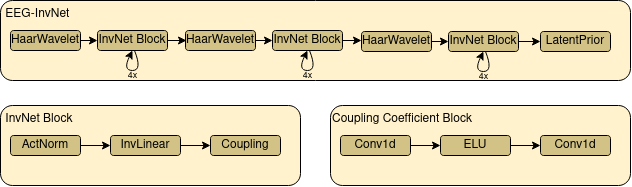
\includegraphics[width=1\linewidth]{images/EEG-InvNet.png}
    \caption[EEG-InvNet architecture]{
\textbf{EEG-InvNet architecture.} Our EEG-InvNet architecture consists
of three stages that operate at sequentially lower temporal resolutions.
Input is two seconds of 21 electrodes at 64 Hz so 21x128 dimensions.
These are downsampled using Haar Wavelets to 42x32 for the first, 84x16
for the second and 164x8 for the last stage. One stage consists of 4
blocks, each block has an activation normalization, an invertible linear
and a coupling layer. The activation normalization and invertible linear
layer act on the channel dimension, so perform the same operation across
channels on timepoint in the feature map. The coupling layer uses two
convolutions with an exponential linear unit activation inbetween.
}
\label{eeg-invnet-fig}
\end{figure}




    We designed an invertible network named EEG-InvNet for EEG Decoding
using invertible components used in the literature, primarily from the
Glow architecture \citep{DBLP:conf/nips/KingmaD18}. Our
architecture consists of three stages that operate on sequentially lower
temporal resolutions. Similar to Glow, the individual stages consists of
several blocks of Activation Normalization, Invertible Linear Channel
Transformations and Coupling Layers, see
\Cref{eeg-invnet-fig}. Between each stage, we downsample by
computing the mean and difference of two neighbouring timepoints and
moving these into the channel dimension. Unlike Glow, we keep processing
all dimensions throughout all stages, finding this architecture to reach
competitive accuracy on pathology decoding. We use one gaussian
distribution per class in the latent space. We experimented with affine
and additive coupling layers, and report results for additive layers as
the restricted expressiveness may make them easier to interpret.

\section{Class Prototypes}\label{methods-class-prototypes}


\begin{figure}[htb]
    \myfloatalign
    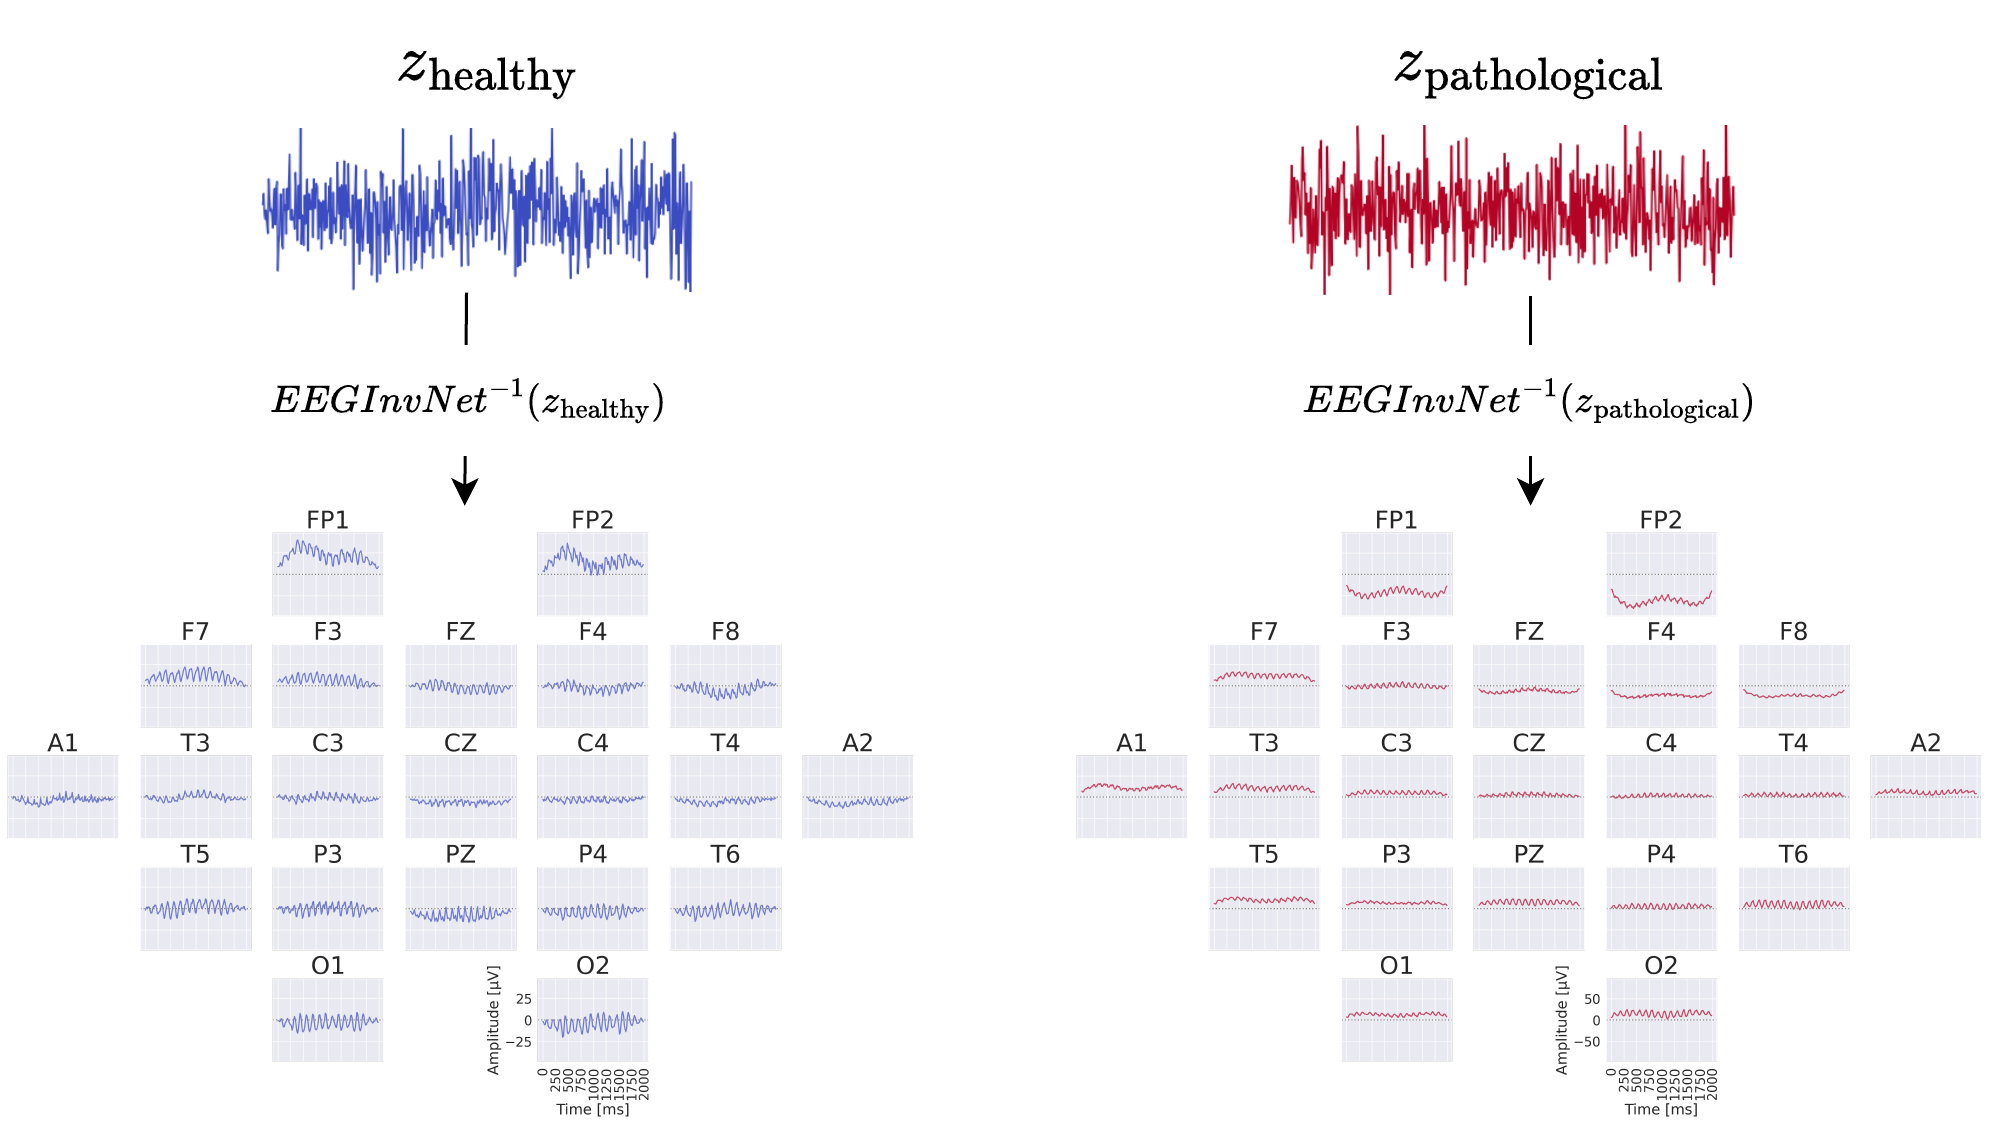
\includegraphics[width=1\linewidth]{images/EEGInvNetClassPrototypes.test.png}
    \caption[EEG-InvNet class prototypes]{
\textbf{EEG-InvNet class prototypes.} Class prototypes are synthesized
by inverting the means $z_\mathrm{healthy}$ and
$z_\mathrm{pathological}$ of the per-class gaussian distributions.
}
\label{eeg-prototypes-fig}
\end{figure}

    In our first visualization, we show the inputs resulting from inverting
the means of the gaussian distributions for each class (see
\Cref{eeg-prototypes-fig}). These can be seen as
prototypical examples of each class and may give hint about the
discriminative features that have been learned. As these are only single
examples, they need to be interpreted cautiously. For example,
individual features within the examples may have a variety of
relationships with the actual prediction function. Consider if a
prototype contains a large alpha-band oscillation at two electrodes,
then these may be indepedendently predictive predictive of that class or
only in combination or even only in some combination with other
features. Nevertheless, the prototypes can already suggest potential
discriminative features for further investigation.

\section{Per-Electrode Prototypes}\label{per-electrode-prototypes}
    

\begin{figure}[h!tb]
    \captionsetup[subfigure]{labelformat=empty}
    \myfloatalign
    \subfloat[]
    {
    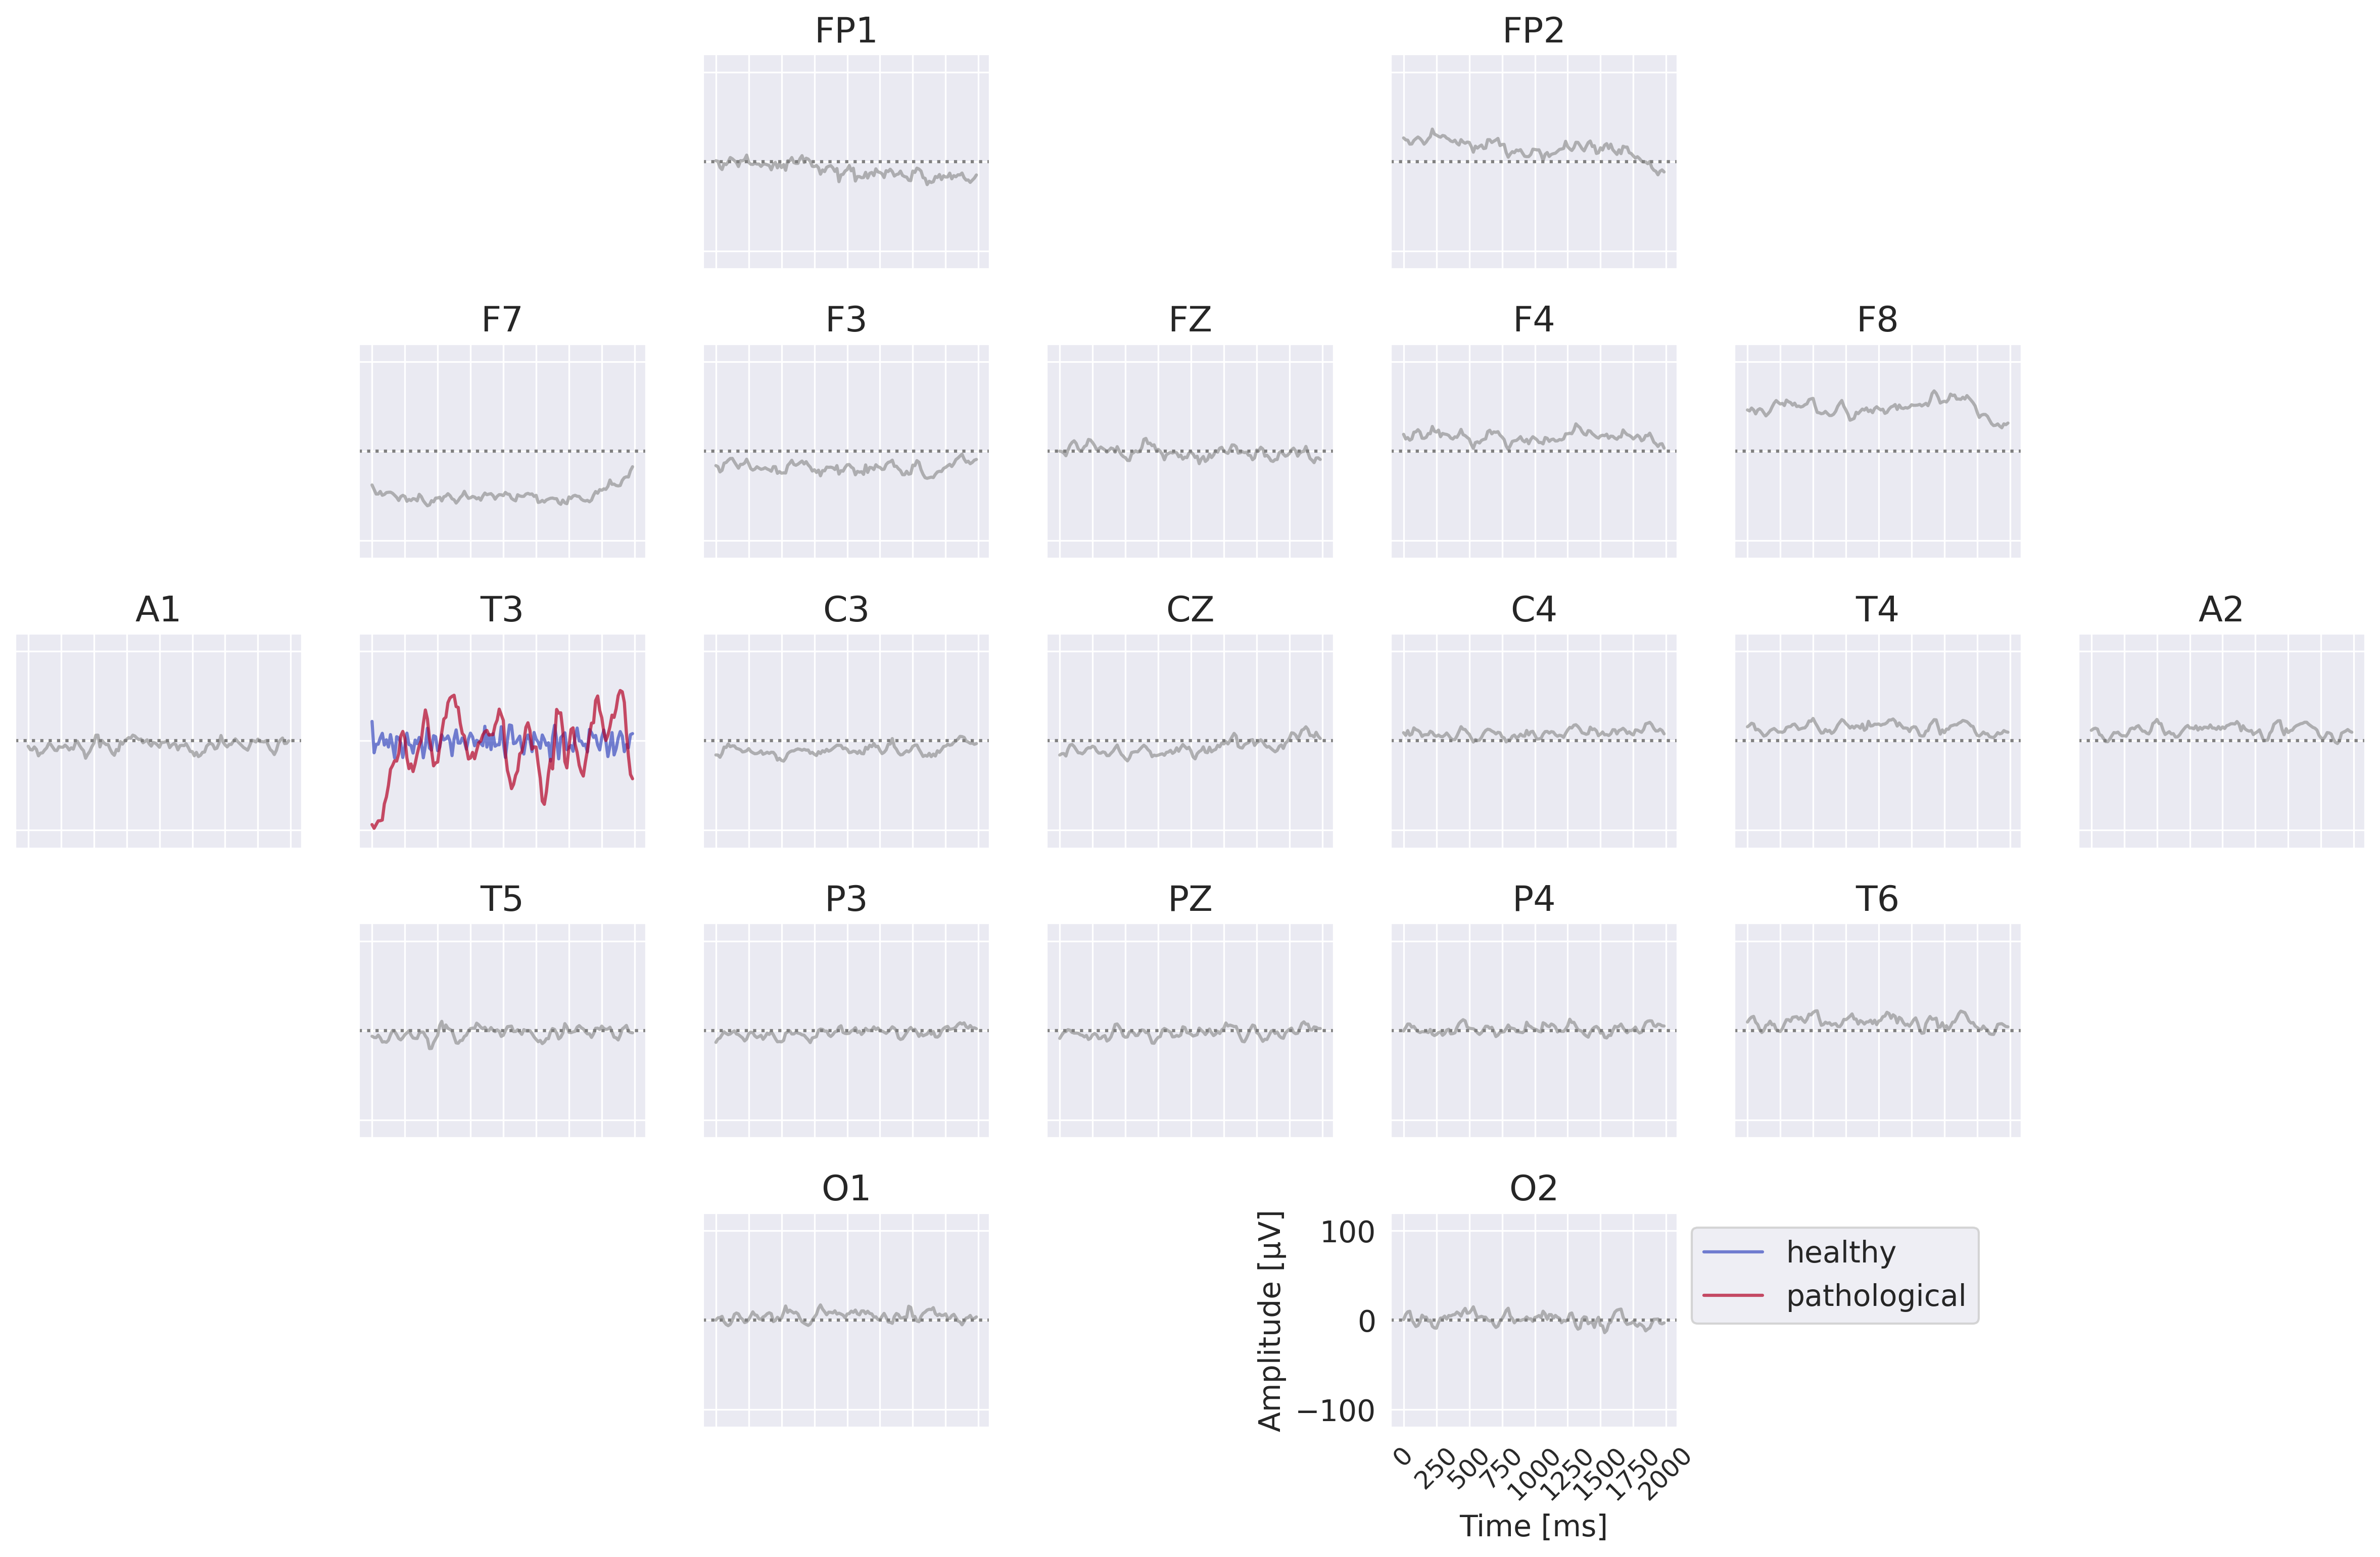
\includegraphics[width=.45\linewidth]{images/marginal-chan-explanation_0.png}} \quad
    \subfloat[] 
    {
        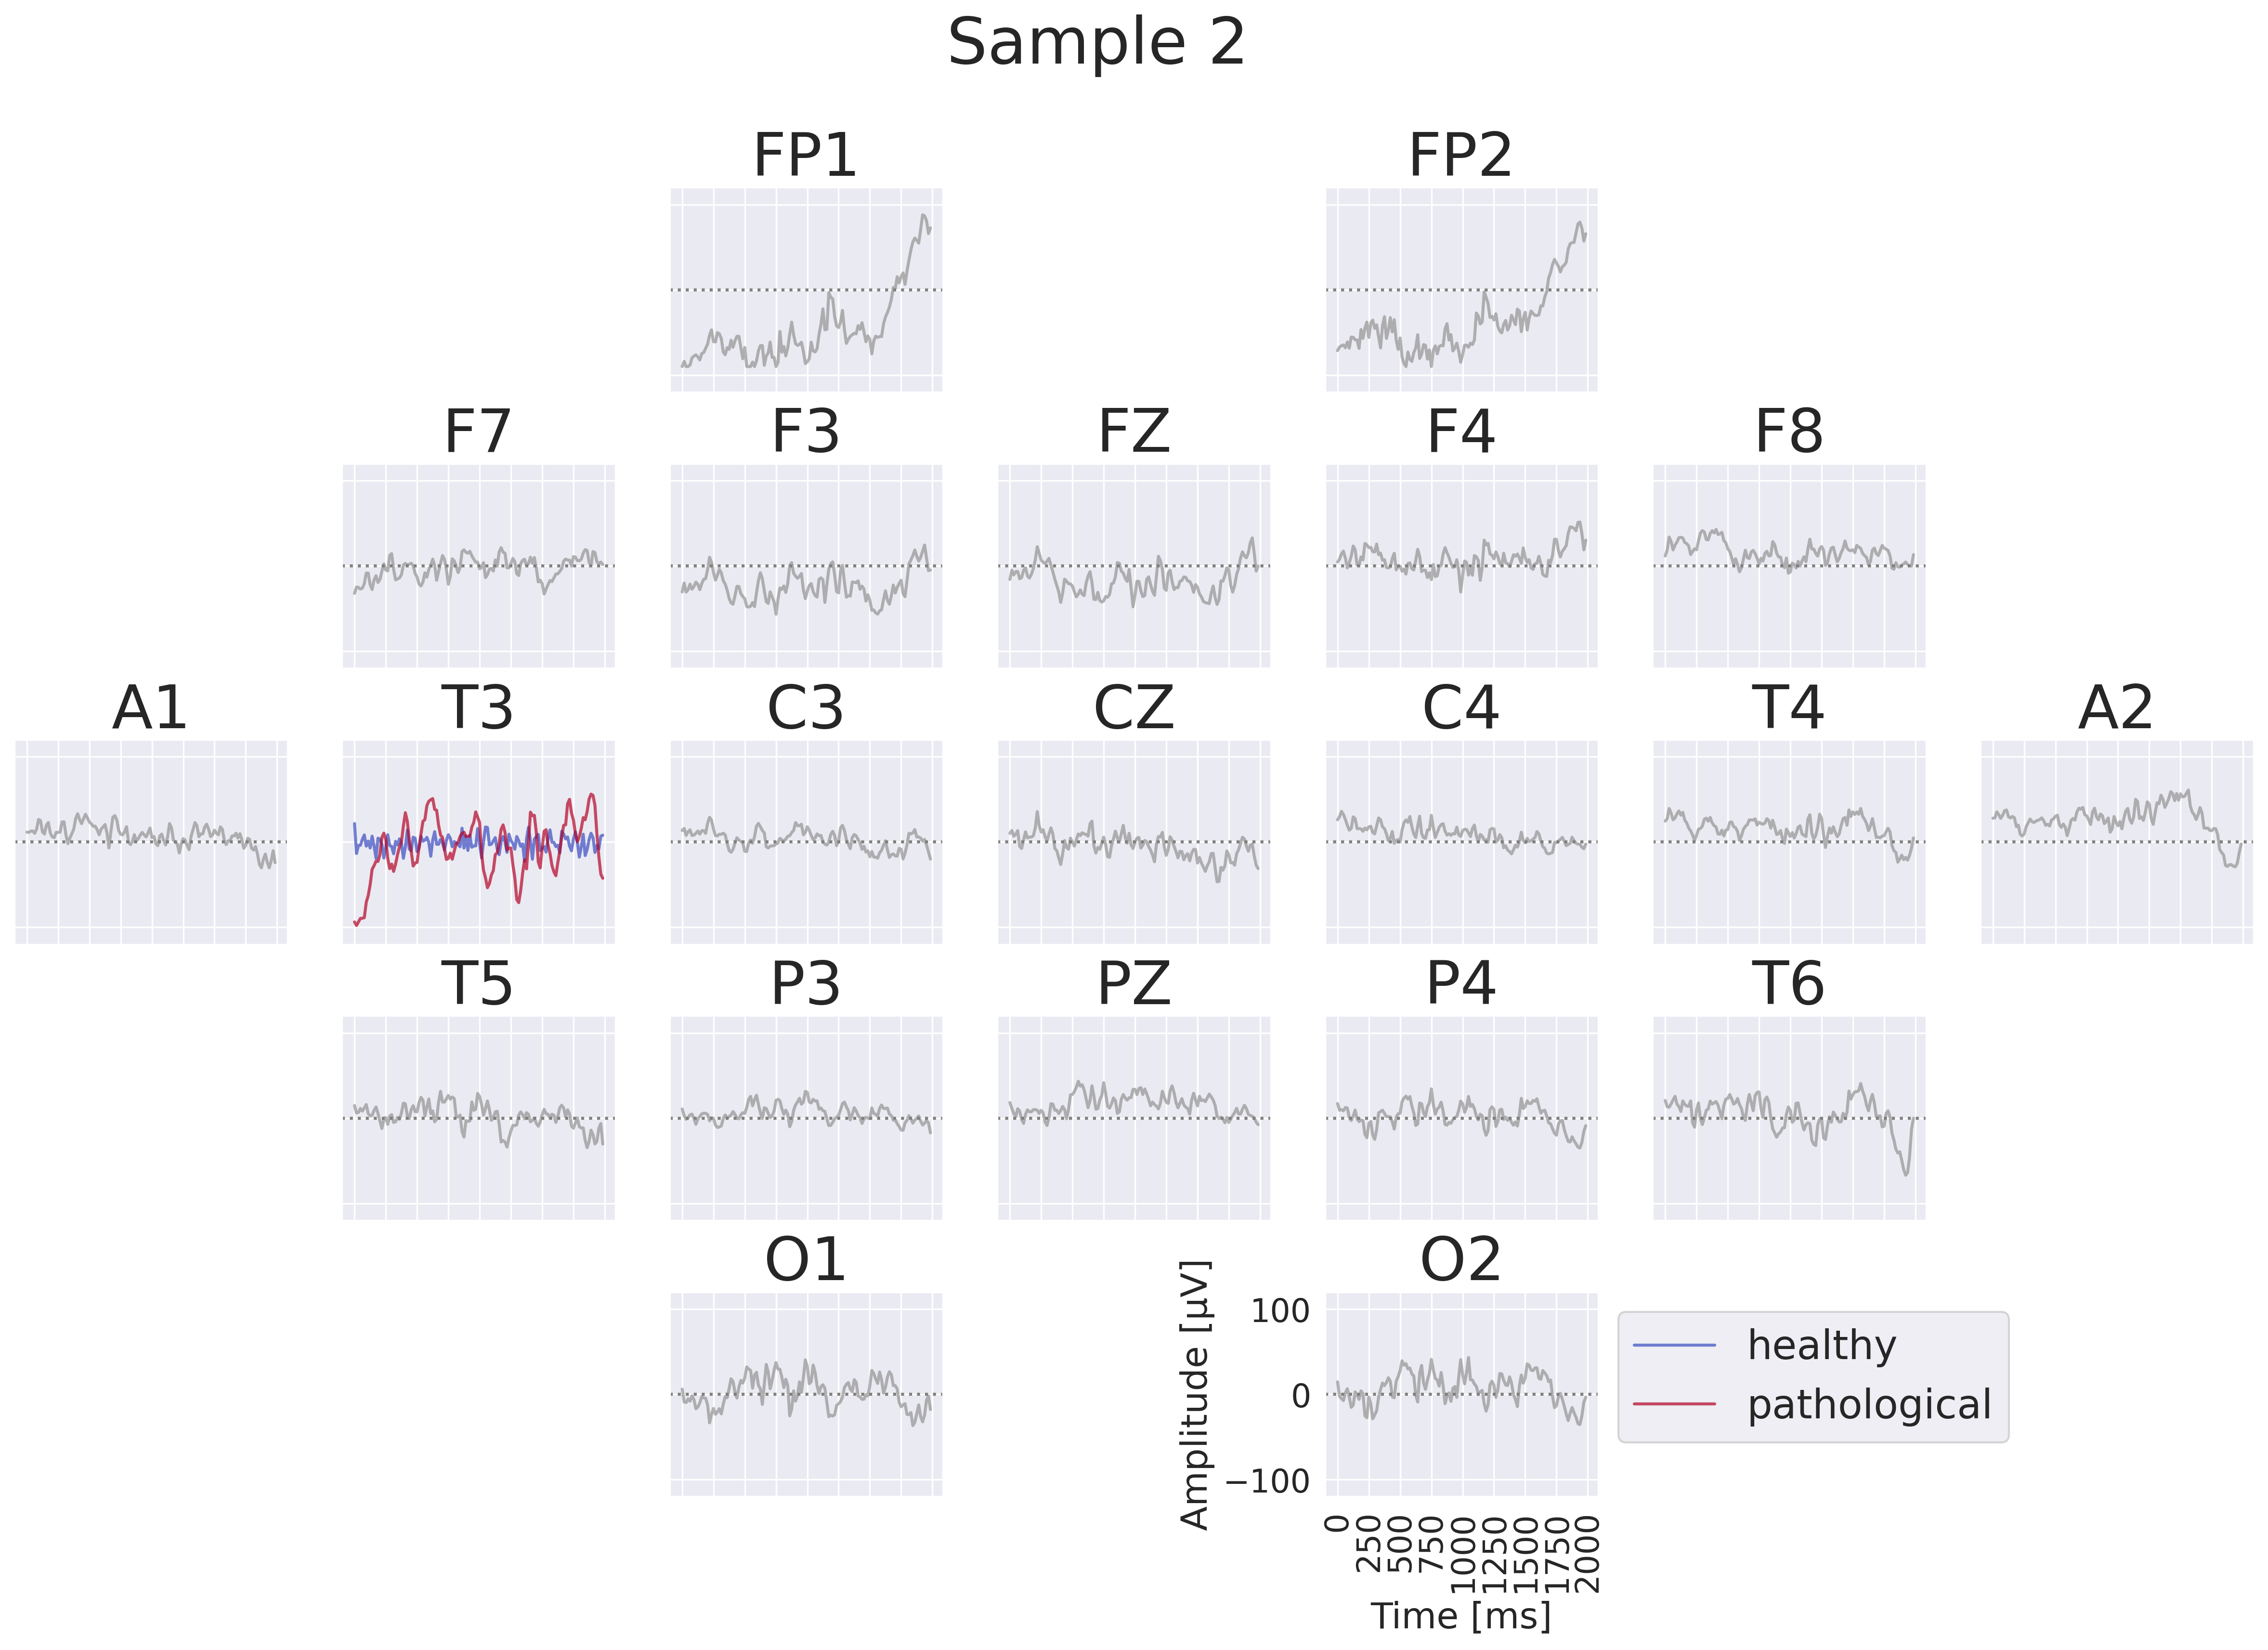
\includegraphics[width=.45\linewidth]{images/marginal-chan-explanation_1.png}} \\
    \subfloat[]
    {
    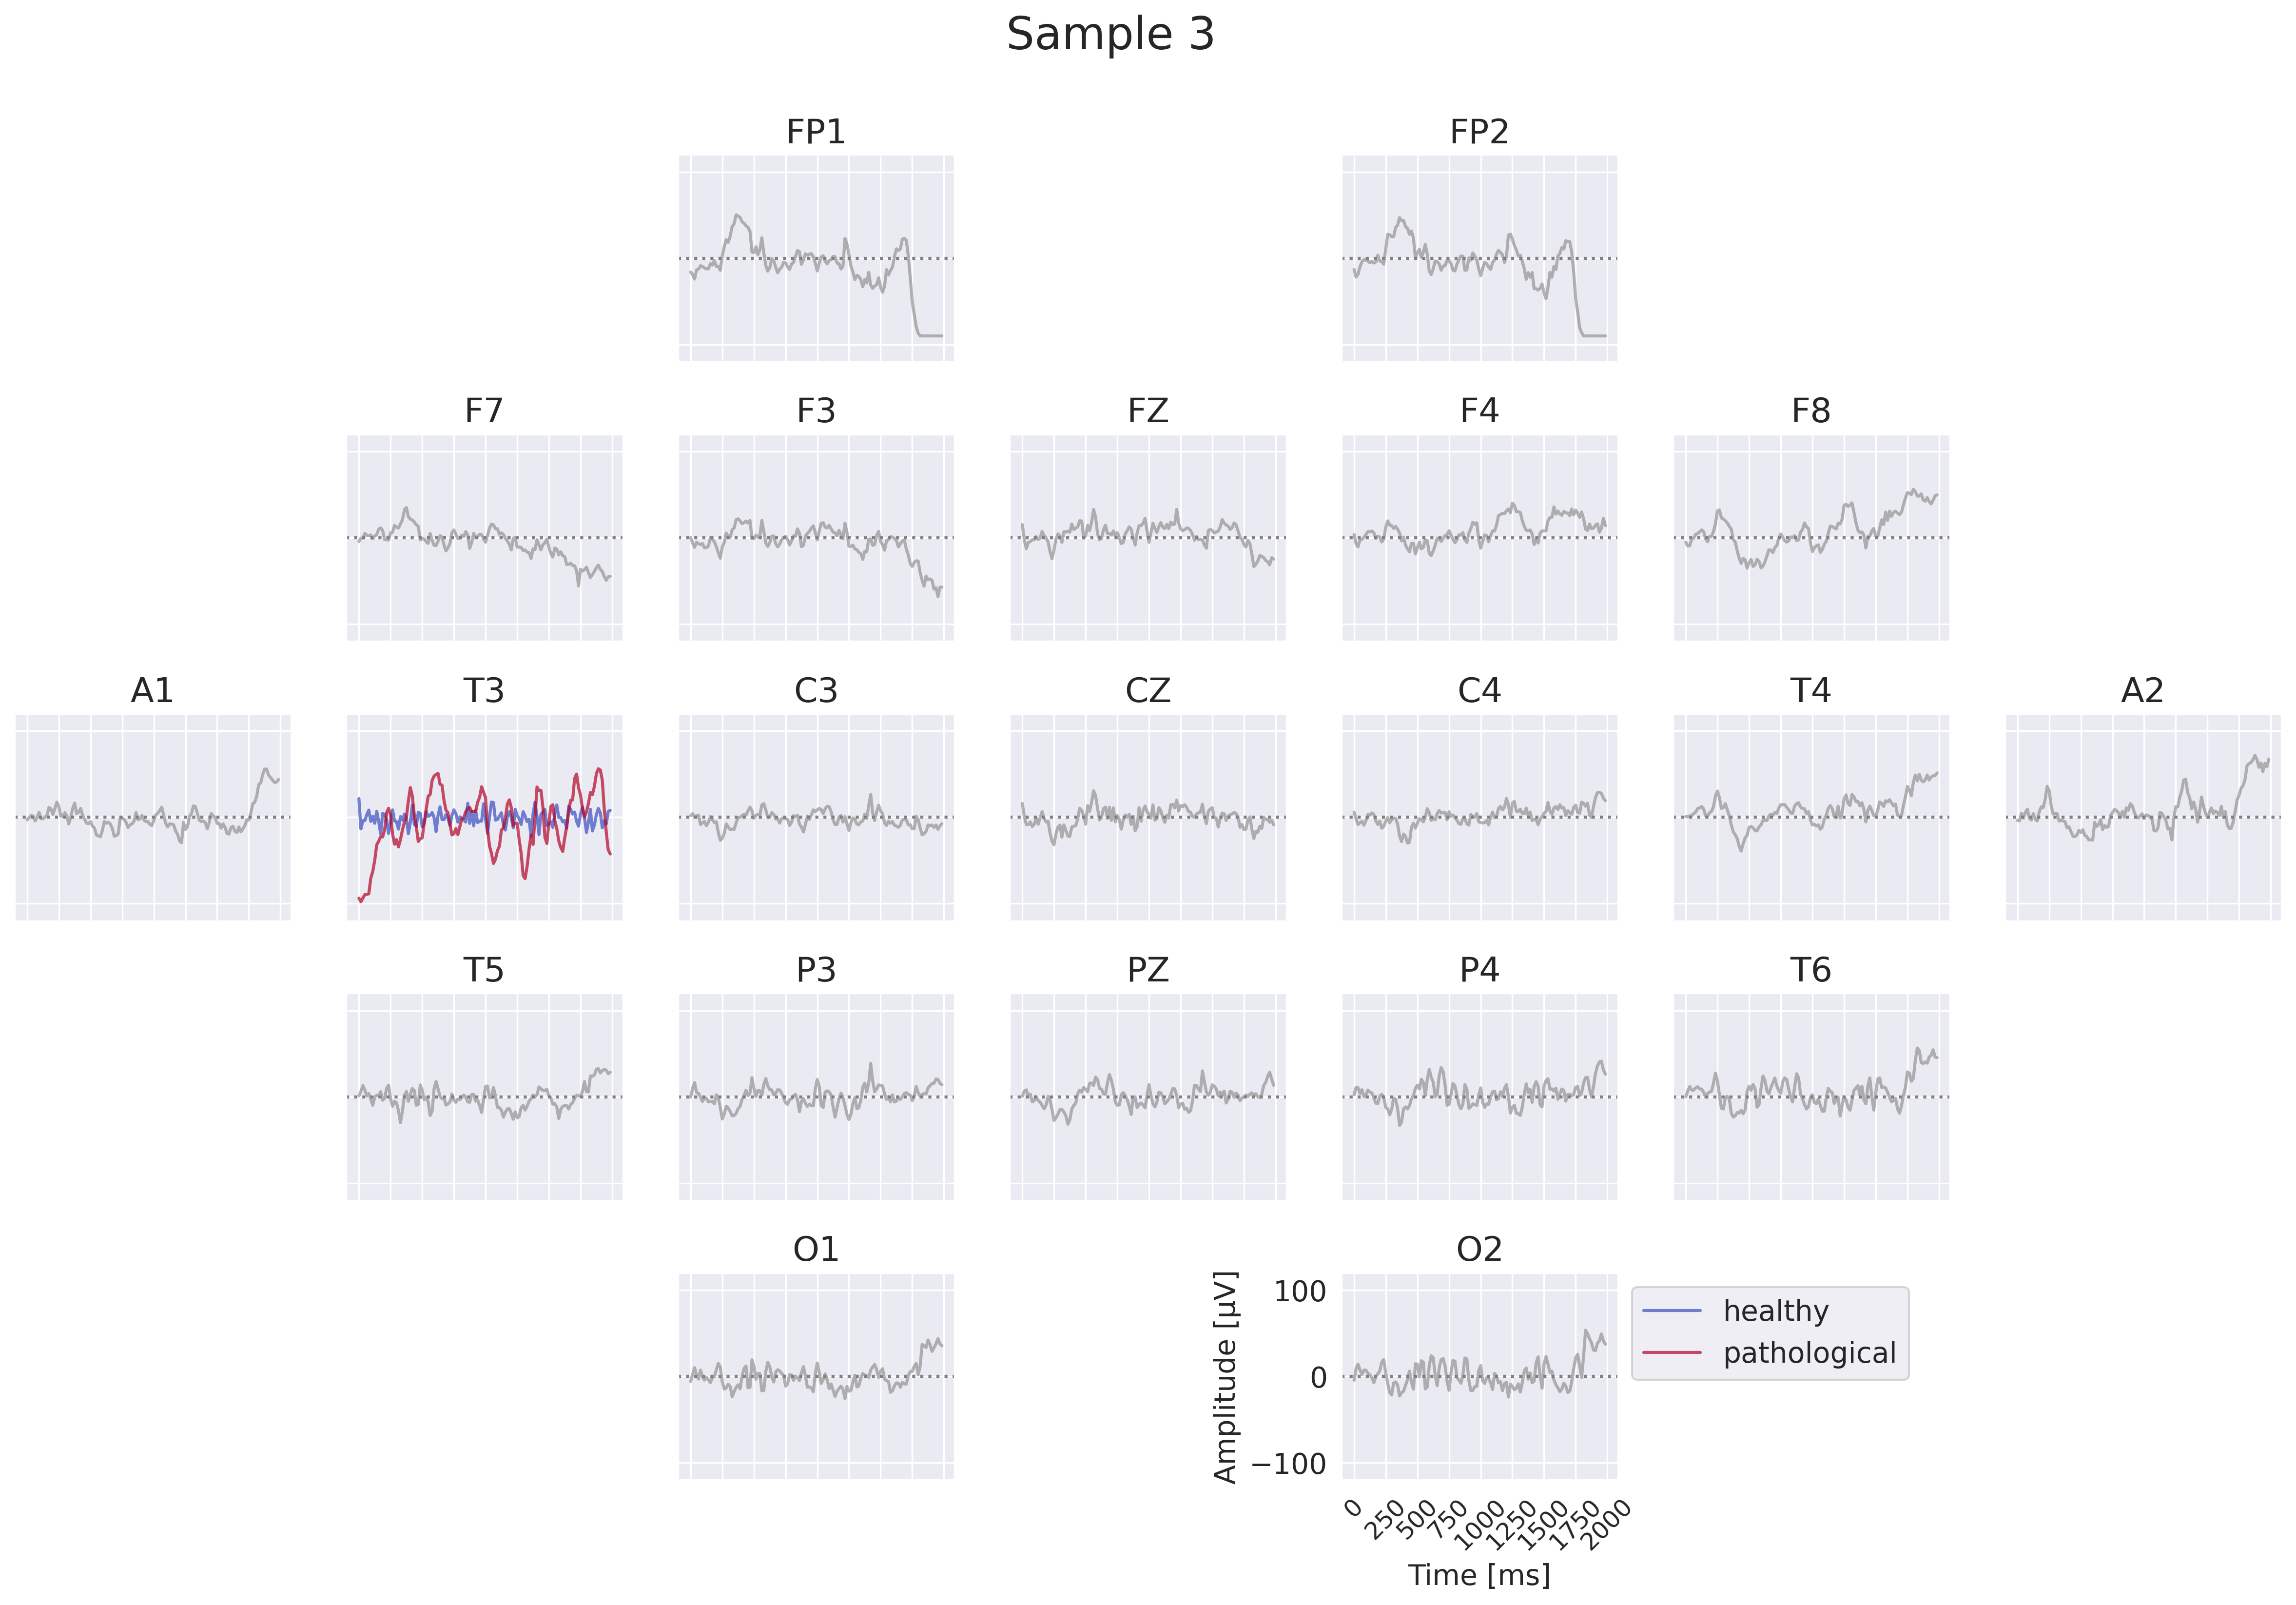
\includegraphics[width=.45\linewidth]{images/marginal-chan-explanation_2.png}} \quad
    \subfloat[]
    {
        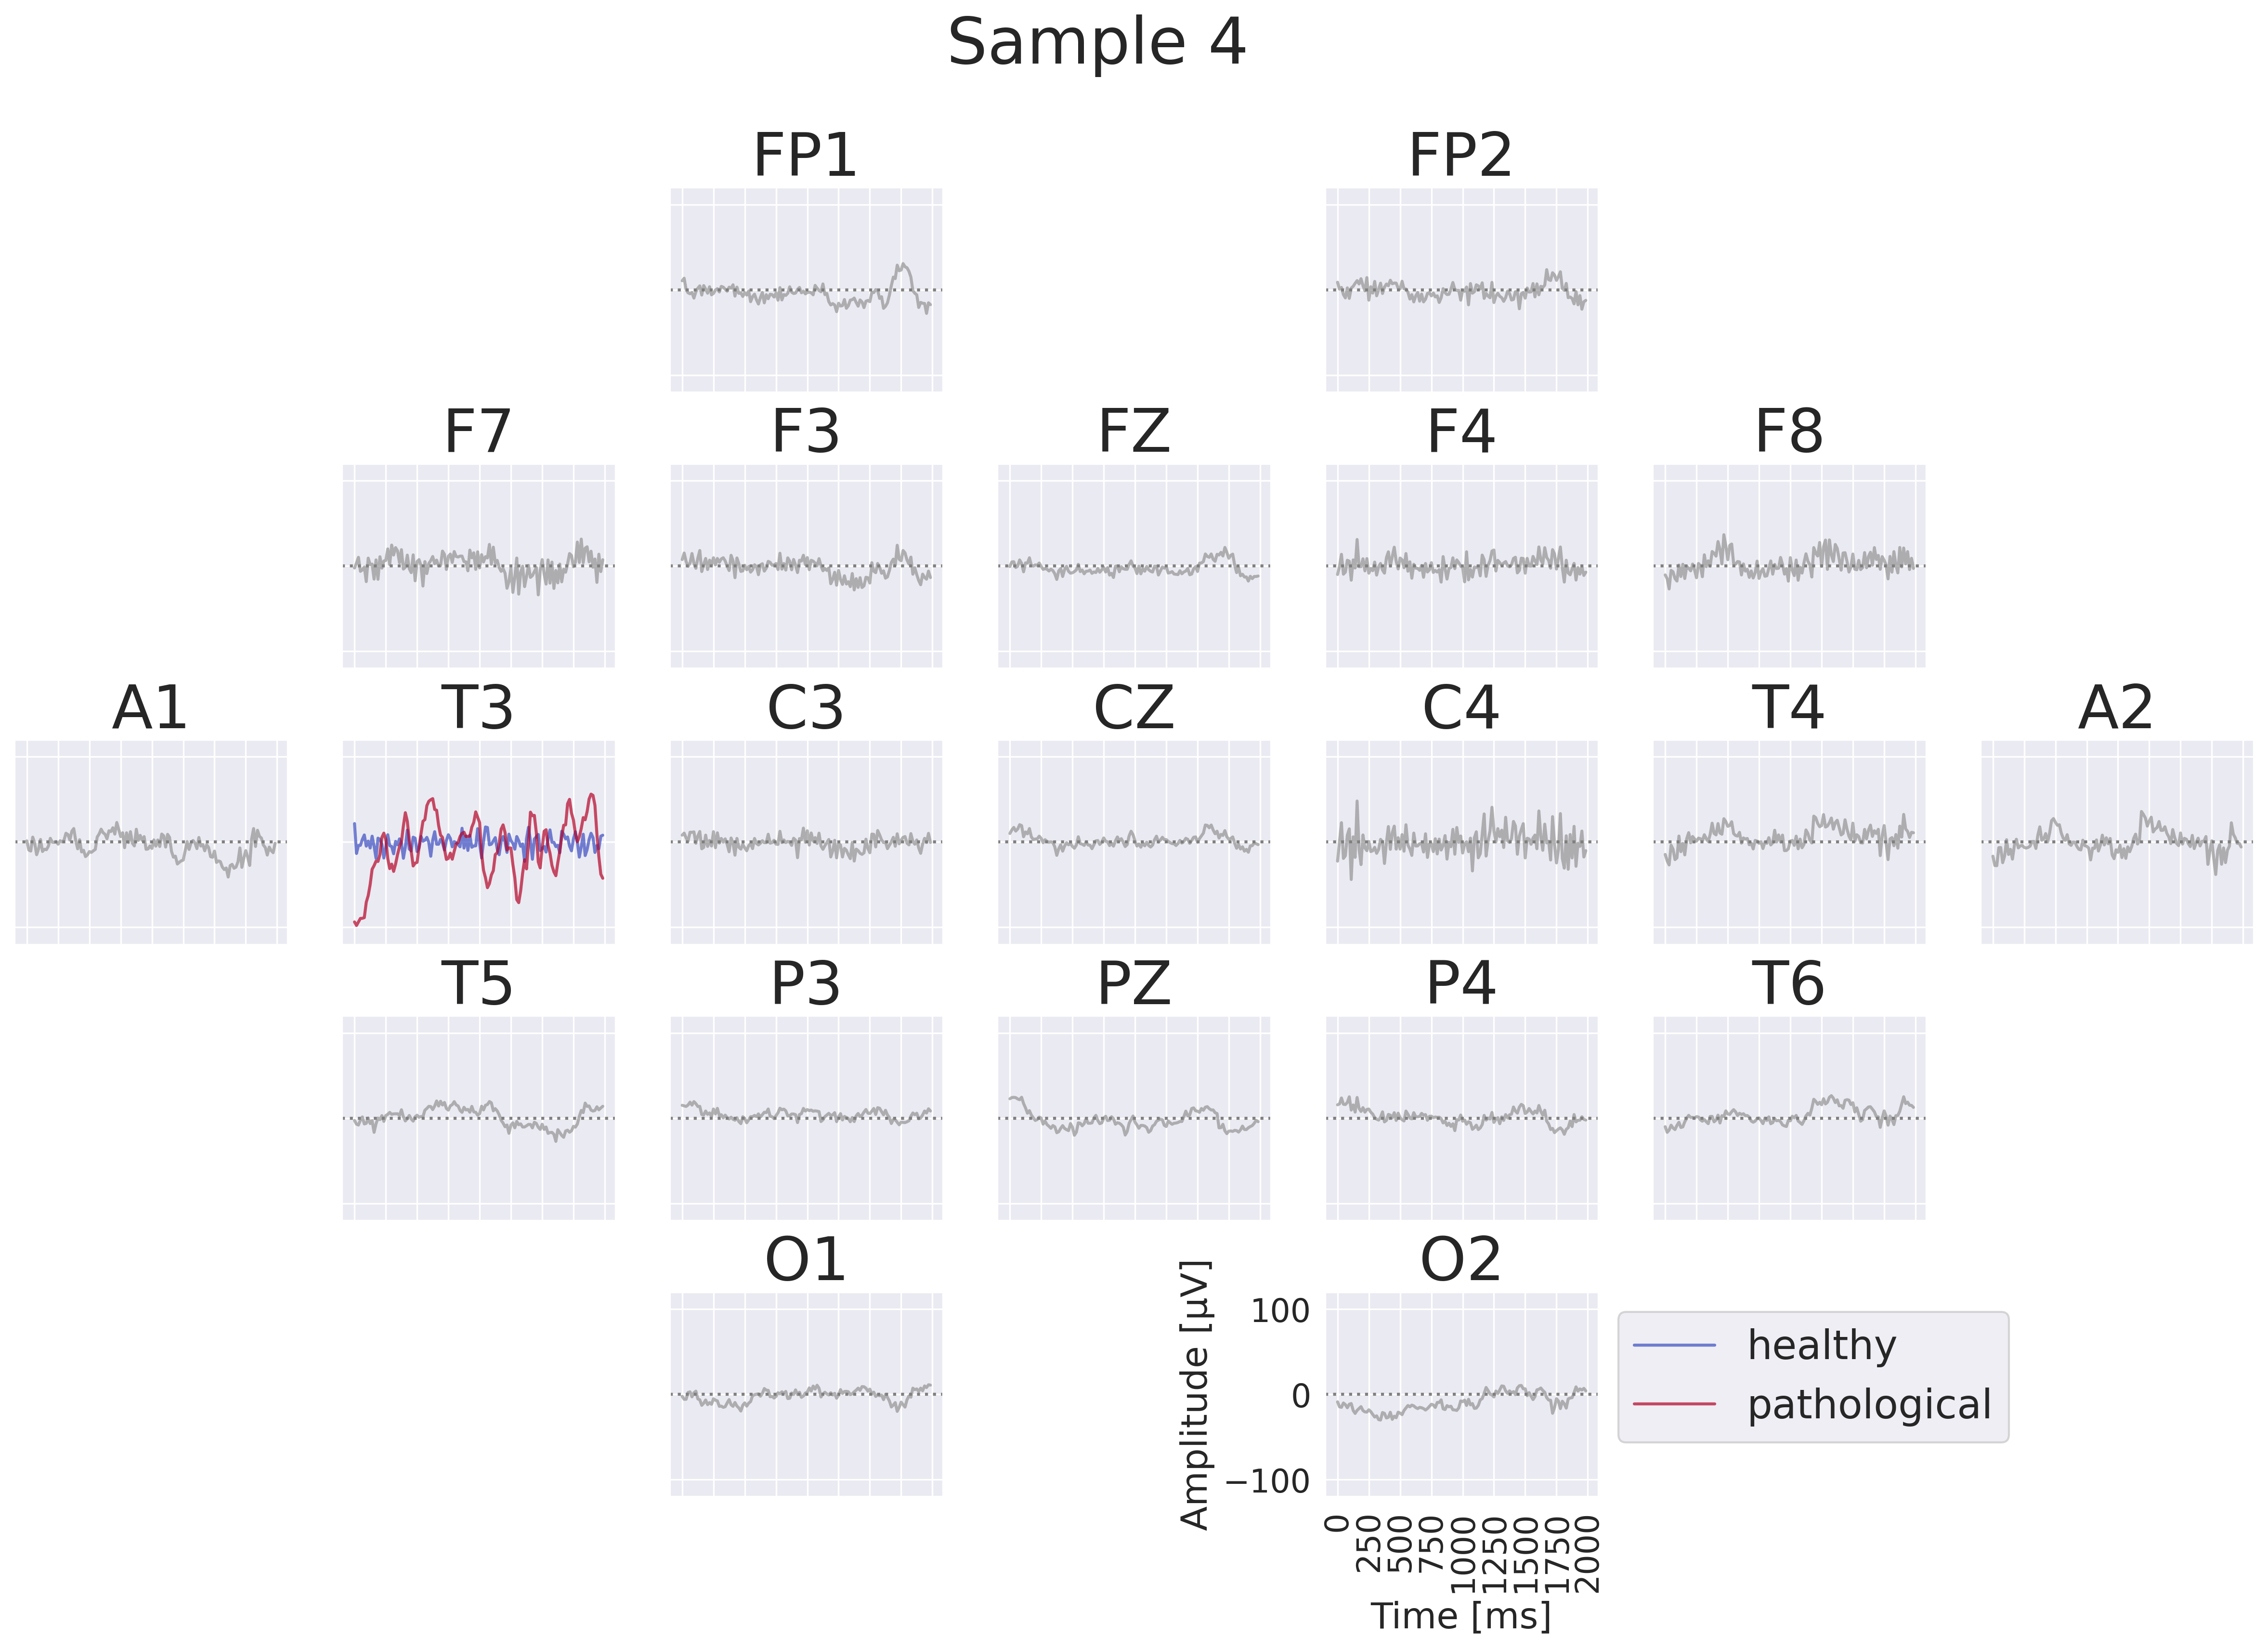
\includegraphics[width=.45\linewidth]{images/marginal-chan-explanation_3.png}} \\
    \caption[EEG-InvNet per-electrode class prototypes]{
    \textbf{EEG-InvNet per-electrode class prototypes.} For getting
per-electrode prototypes, synthetic class-specific signals for one electrode are optimized to yield high predicted class probabilities for any signals at other electrodes.  Signals at other electrodes are sampled from training
data. In the example, prototypes for T3 for the healthy and pathological
class are learned, four samples for remaining electrodes are shown. In
practice, a much larger number of samples would be used. Class signal
probabilities are marginalized over the non-optimized channels as
explained in text.
    }\label{invnet-marginal-chan-explanation-fig}
\end{figure}


    One way to get more interpretable prototypes is to synthesize them per
electrode. Here, we synthesize a signal $x^*_{e_k}$ for a specific
electrode $e_k$ such that the class prediction is high for one class,
independent of the signals at the other electrodes (see
\Cref{invnet-marginal-chan-explanation-fig}). So for
electrode $e_k$ and class $c_i$, we aim to optimize the signal
$x^*_{e_k}$ by maximizing the marginals
$p(x^*_{e_k}|c_i)=\int p(x|c_i;x_{e_k}=x^*_{e_k}) dx$ (generative
loss) and
$p(c_i|x^*_{e_k})=\frac{p(x^*_{e_k}|c_i)}{\sum_j p(x^*_{e_k}|c_j)}$
(classification loss). To approximate this, we sample $n$ signals
$x_l$ of the training distribution and replace the signal
$x_{l,e_k}$ of the electrode $e_k$ we are synthesizing by the
optimized $x^*_{e_k}$. This leads to
$p(x^*_{e_k}|c_i)\approx\sum_{l=1}^n p(x_l|c_i;x_{l,e_k}=x^*_{e_k})$.
While being only a coarse approximation, this already yields insightful
visualizations. For the classification loss, when computing
$p(c_i|x^*_{e_k})$, we found it helpful to first divide the log
probabilities $\log p(x_l|c_i;x_{l,e_k}=x^*_{e_k})$ by the learned
temperature $t$ of the classifier:
$\log p_\mathrm{clf}(x^*_{e_k}|c_i)=\mathrm{logsumexp}\left(\frac{\log p(x_l|c_i;x_{l,e_k}=x^*_{e_k})}{t}\right)$.
Otherwise, $\sum_n p(x_n|c_i;x_{n,e_k}=x^*_{e_k})$ may be dominated by
just a few samples when computing $p(c_i|x^*_{e_k})$. We only apply
this for the classification loss $p(c_i|x^*_{e_k})$, not the
generative loss $p(x^*_{e_k}|c_i)$.

\section{EEG-CosNet}\label{methods-eeg-cosnet}
    

\begin{figure}[htb]
    \captionsetup[subfigure]{labelformat=empty}
    \myfloatalign
    \subfloat[]
    {
    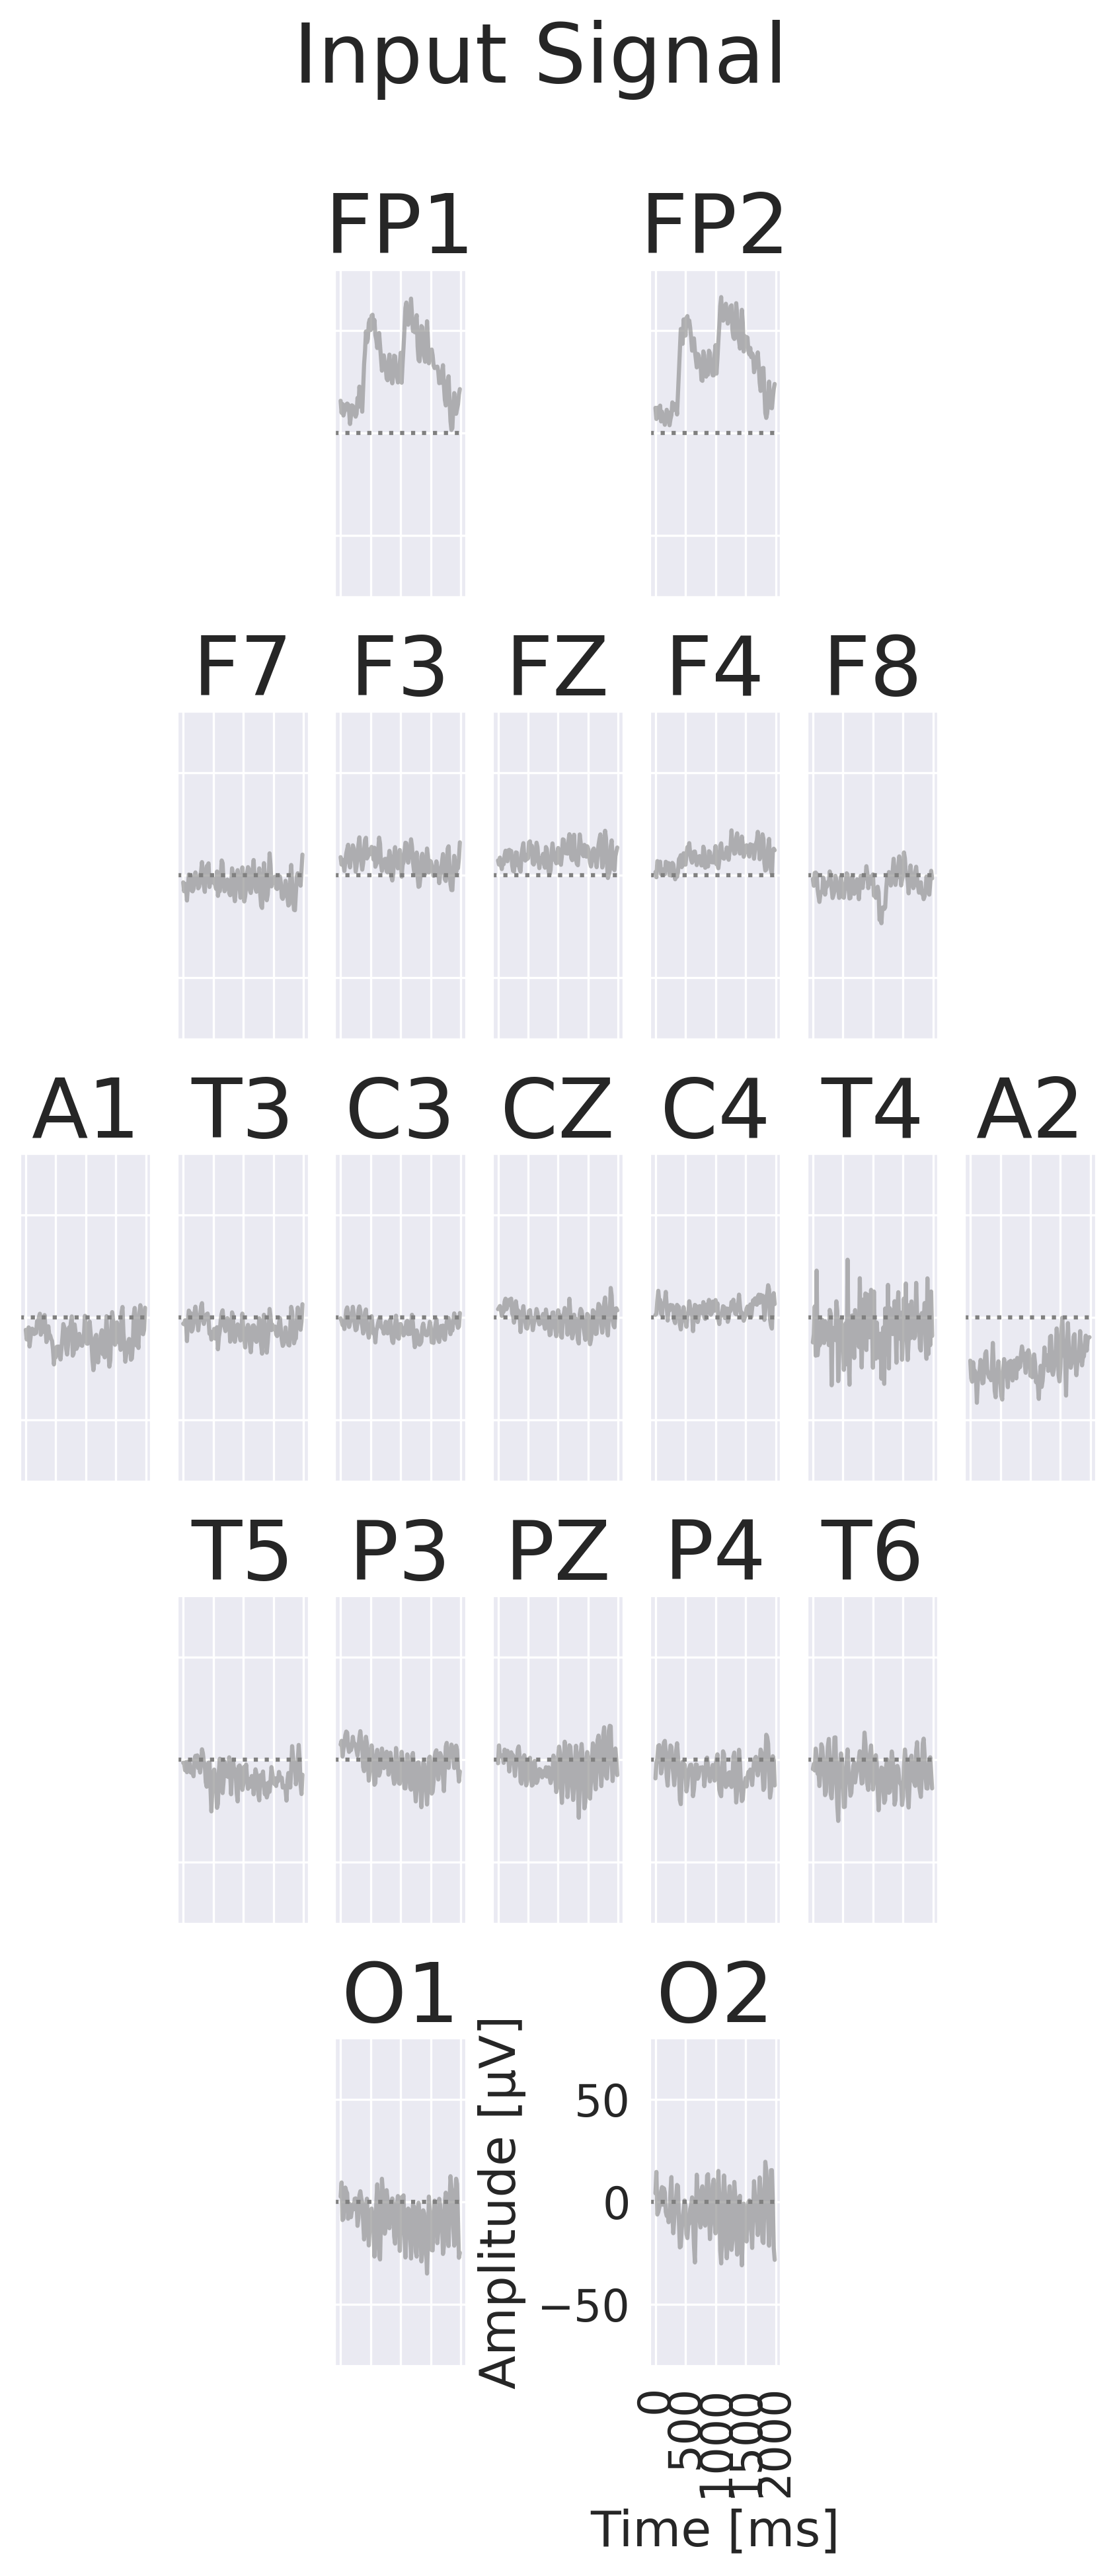
\includegraphics[width=.235\linewidth]{images/cos-net-example-input.png}} \quad
    \subfloat[]
    {
        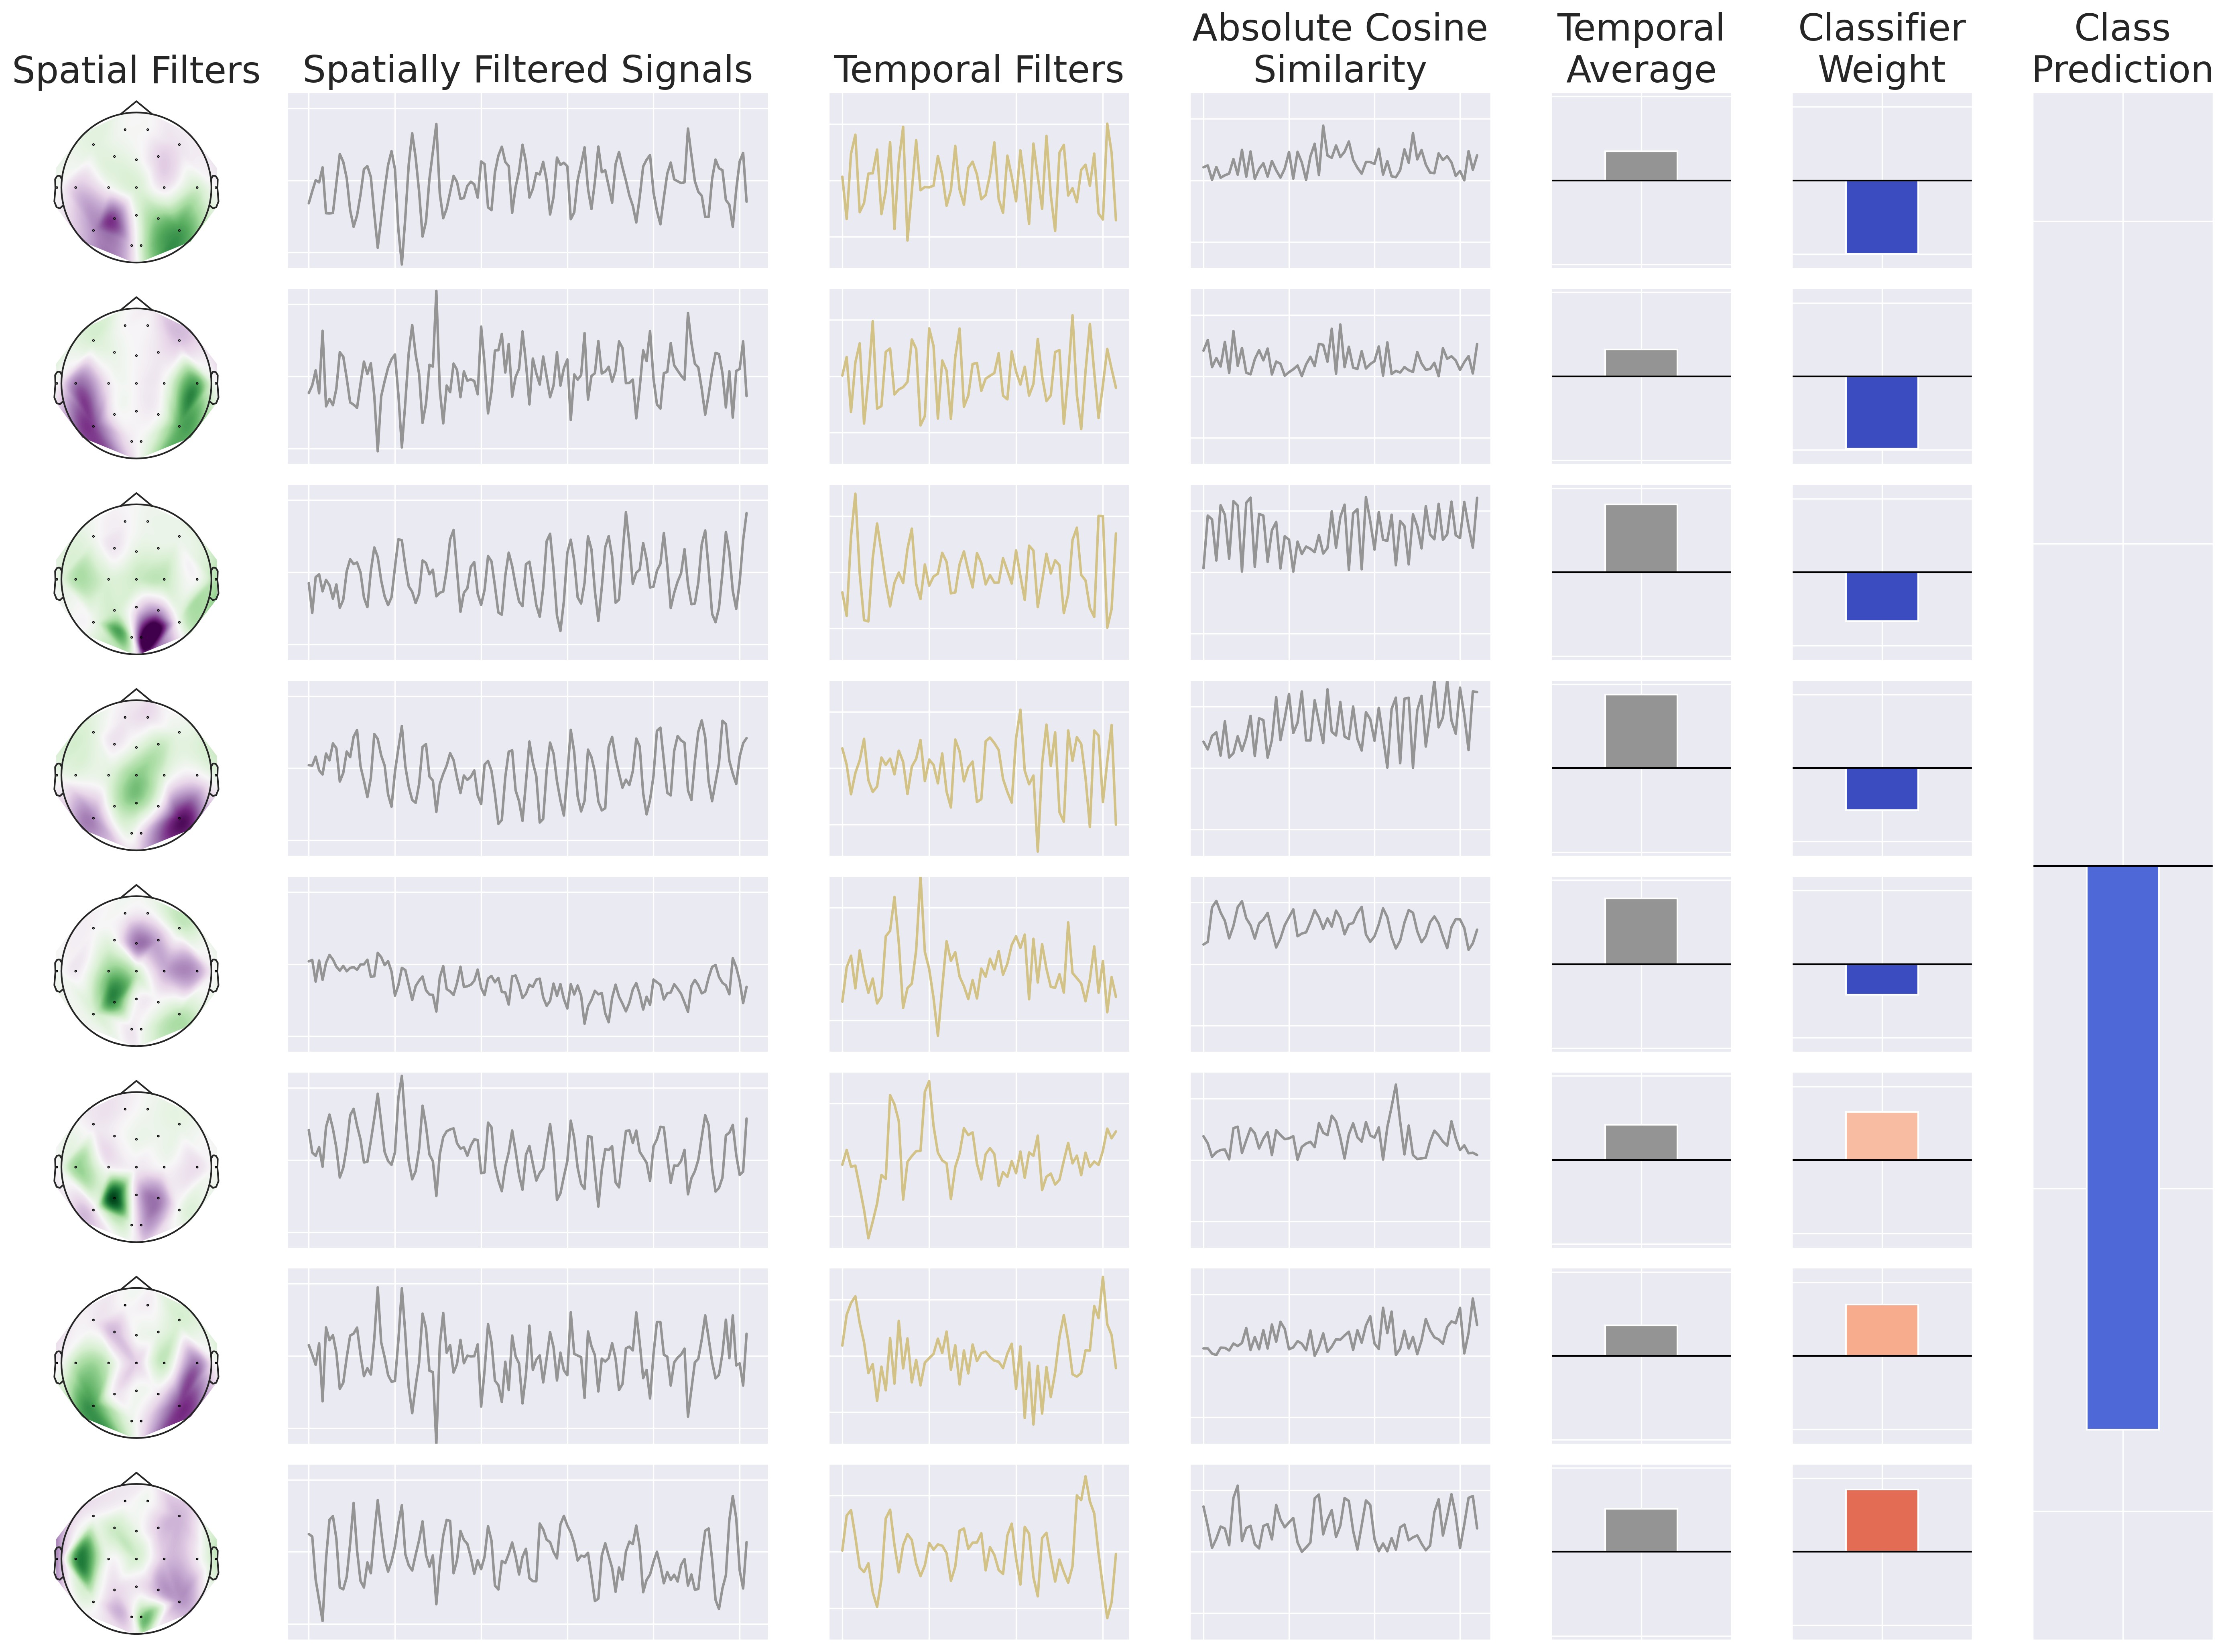
\includegraphics[width=.72\linewidth]{images/cos-net-example-processing.png}} 
    \caption[Example processing of the EEG-CosNet.]{
    \textbf{Example processing of the EEG-CosNet.} Example EEG input on the
left, then processing steps on the right: spatial filtering, absolute
cosine similarity with temporal filters, temporal averaging, then
weighting with linear classifier weights for class prediction. Note the
EEG-CosNet in this visualization only uses 8 filters, whereas later we
will use 64 filters.
}\label{cos-net-example-fig}
\end{figure}


    Finally, we also implemented a small convolutional network EEG-CosNet
that we designed to be directly interpretable. We tried to distill the
trained EEG-InvNet into the EEG-CosNet by training the EEG-CosNet using
the EEG-InvNet class probabilities as the targets for the classification
loss $L_\textrm{class}$. Our EEG-CosNet consists of just three steps
(see \Cref{cos-net-example-fig} for an example computation):


\begin{align*}
    \intertext{\textbf{Spatial Filtering}}
    h_1 &= W_s^Tx && \codecomment{\text{Apply spatial filter weights } W_s \text{ to  inputs }} \\
    \intertext{\textbf{Feature construction}}
    h_2 &= |\mathrm{cos\_sim}(h_1, \mathrm{filters})| && \codecomment{\text{Abs. moving cosine similarity with temporal filters}} \\
    h_3 &=\frac{\sum_t (h_2)}{n_\mathrm{times}} && \codecomment{\text{Average over timepoints in trial}} \\
    \intertext{\textbf{Classification}}
    h_4 &= W_c^Th_3 && \codecomment{\text{Apply classifierweights } W_c \text{ on these features }} \\
p(\mathrm{c_\mathrm{path}}|h_4) &= \frac{1}{1 + \sum_j e^-h_{4}} && \codecomment{\text{Compute sigmoid to get pathological probability}} \\
\end{align*}

Steps 1 and 2 yield spatiotemporal patterns that can be visualized as
waveforms and scalp plots, and that are weighted by the linear
classifier for the respective classes. We chose cosine similarity to
ensure that high output values correspond to spatially filtered signals
that resemble the corresponding temporal filter. The spatial filter
weights and linear classifier weights can be made even more
interpretable through transforming the discriminative weights into
generative patterns by multiplying them with the covariance of the
electrodes/averaged absolute cosine similarities after training, see
\citet{haufe_interpretation_2014} for a discussion on this
technique. We use 64 spatiotemporal filters with temporal length 64
corresponding to one second at 64 Hz.


\begin{openbox}
\item How well can the EEG-InvNet perform on EEG Pathology decoding?
\item What features can the EEG-InvNet reveal?
\item How well can the EEG-CosNet approximate the EEG-InvNet?
\item What features can the EEG-CosNet reveal?
\end{openbox}
